% Created 2015-04-27 Mon 15:18
\documentclass[11pt]{article}
\usepackage[utf8]{inputenc}
\usepackage[T1]{fontenc}
\usepackage{fixltx2e}
\usepackage{graphicx}
\usepackage{longtable}
\usepackage{float}
\usepackage{wrapfig}
\usepackage{rotating}
\usepackage[normalem]{ulem}
\usepackage{amsmath}
\usepackage{textcomp}
\usepackage{marvosym}
\usepackage{wasysym}
\usepackage{amssymb}
\usepackage{hyperref}
\tolerance=1000
\author{Ista Zahn}
\date{}
\title{RCE Quick-Start}
\hypersetup{
  pdfkeywords={},
  pdfsubject={},
  pdfcreator={Emacs 24.5.1 (Org mode 8.2.10)}}
\begin{document}

\maketitle
\tableofcontents


\section{What is the RCE}
\label{sec-1}
The Research Computing Environment (RCE) is a large powerful computer cluster that you can use for computations that are too large to be conveniently done on a personal computer. The RCE is available to researchers at Harvard and MIT. 

To obtain an RCE account send an email to \url{mailto:help@iq.harvard.edu}. You will receive a response asking you several questions about your requirements (e.g., if you need backups, how much data storage space you need). For details on the services provided and limitations and restrictions of the service refer to \url{http://projects.iq.harvard.edu/user-services/research-computing-environment-sla}

You can use the RCE in one to two primary ways:
\begin{description}
\item[{Interactive jobs}] Run your computation as you would on your PC, but on a much more powerful machine with up to 24 CPU cores and up to 256Gb of memory.
\item[{Batch jobs}] Run your computation in the background using up to several hundred computers at once.
\end{description}

Interactive jobs are good for memory intensive computations that may be unfeasible on your personal computer due to hardware limitations. Batch jobs are good for computations that can be run in parallel and/or computations that you expect to run for long periods of time.


\section{Accessing the RCE}
\label{sec-2}
You can access the RCE using the \href{http://projects.iq.harvard.edu/rce/nx4_installation}{nomachine} remote desktop software, or via the command line using \texttt{ssh}. If you are a command line wizard and only need to run batch jobs \texttt{ssh} is the way to go; for most of us however \texttt{nomachine} is a much more useful way to access the RCE. It allows you to interact with the applications on the cluster much as you interact with applications on your local computer. To get started, download the NoMachine client for your operating system: \href{http://downloads.hmdc.harvard.edu/nx/4/nomachine-client-windows-latest.zip}{Windows}, \href{http://downloads.hmdc.harvard.edu/nx/4/nomachine-client-osx-latest.dmg}{OSX}, \href{http://downloads.hmdc.harvard.edu/nx/4/nomachine-client-linux-latest.zip}{Linux}. 

After downloading, Windows users should right-click on the \texttt{nomachine-client-windows-latest.zip} file and choose \texttt{Extract to here}. Open the \texttt{NoMachine Client} folder and double-click on the .Exe files to start the installation\footnote{Note: The Windows zipfile contains the NX client, plus optional font packages. HMDC recommends installing all font packages, though this is not required.}. Mac users should double-click on the \texttt{nomachine-client-osx-latest.dmg} and double-click on the installer package to begin the installation.

Once you have installed the NoMachine software you should launch the NoMachine application and set up your login credentials. Once the application launches click \texttt{Continue}, then click \texttt{Click here to create a new connection}. Keep clicking \texttt{Continue} until you get to the Hosts screen. Fill in the Host field with \texttt{rce.hmdc.harvard.edu}. Keep clicking \texttt{Continue} until you get to the Name screen. fill in the Name field with \texttt{RCE6} and click \texttt{Done}.

Once you have configured NoMachine you should test it out to make sure you can connect to the RCE. Click on the \texttt{RCE6} entry and then click \texttt{Connect}. Fill in the user name and password fields with your RCE user name and password. On the following screen click on \texttt{New virtual desktop or custom session}, then click on \texttt{Create a new virtual desktop} and click \texttt{Continue}. You should see an instruction screen; click \texttt{OK} and you should see your RCE desktop, which will look something like this:

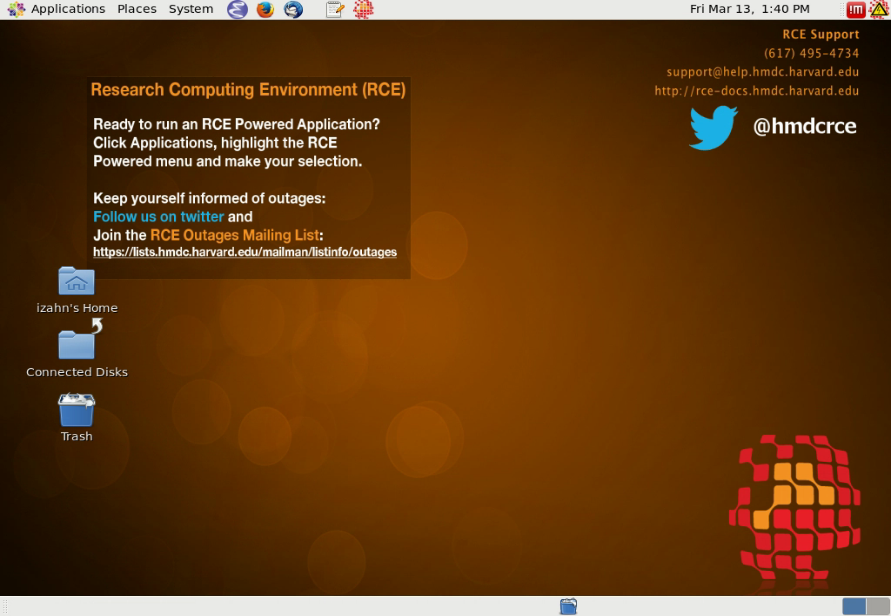
\includegraphics[width=.9\linewidth]{images/rceDesktop.png}

If you have any difficulties installing NoMachine, detailed documentation is available at \url{http://projects.iq.harvard.edu/rce/nx4}; if you do not find a solution there send and email to \url{mailto:help@iq.harvard.edu} and someone will assist you.

\section{Power at your fingertips}
\label{sec-3}

You can run applications on the RCE \emph{interactively} or using the \emph{batch} system. Often the first thing you will want to determine before using the RCE for a particular computation is whether your computation is more suitable for running in the interactive nodes or on the batch nodes. If you simply want a more powerful version of your PC (e.g., more memory, more CPUs) then the interactive nodes are what you want. If you want to split your task up into hundreds of pieces and run each piece simultaneously, then you want the batch modes.

More specifically, the RCE provides three levels of service:
\begin{description}
\item[{Login nodes}] Provides access to a desktop environment (similar to Remote Desktop) from which you can launch applications. The login nodes should not be used for computationally intensive jobs; the main function of the login nodes is to provide access to the interactive and batch nodes. You access the login nodes using the NoMachine client, as described in \hyperref[sec-2]{Accessing the RCE}.
\item[{Interactive nodes}] Interactive nodes allow you to run applications on very powerful computers. You can launch applications on the interactive nodes from the login node desktop using the \texttt{Applications -{}-> RCE Powered Applications} menu. Applications launched from this menu will run on more powerful machines with large memory resources (up to 256GB) and up to 24 CPU cores.
\item[{Batch nodes}] Where interactive nodes give you access to a single very powerful computer, batch nodes provide a swarm of hundreds of small computers. You can run your computation in parallel on each of them, which can provide dramatically reduced compute time for many applications. You access the batch nodes using the \emph{command line} which you can access by starting a terminal application from the  \texttt{Applications -{}-> Accessories -{}-> terminal} menu.
\end{description}

\section{Project folders \& shared space}
\label{sec-4}
When your RCE account was created a home folder was set up for you, with \emph{Documents}, \emph{Downloads}, \emph{Desktop} and other common sub-directories. However you can only store a maximum of 5Gb in your home folder. For larger projects you should use a \emph{project folder}; one was probably set up for you when your account was activated. There is a shortcut in your home directory named \emph{shared\_space}, which will contain any project folders you have access to. You should store large data sets and other large or numerous files in these project folders.

Project space can be used privately, or shared with collaborators (hence the name, "shared space"). Because our researchers bring confidential data to the RCE, we keep all project space separate from your home directory. There are four types of project space:
\begin{itemize}
\item Project space with long-term backups
\item Project space without long-term backups
\item Confidential project space with long-term backups
\item Confidential project space without long-term backups
\end{itemize}
When you apply for an RCE account, you are asked which category would best suit your needs. Therefore, you should know ahead of time if your data is rated as confidential information by your IRB.

For more details on project folders refer to \url{http://projects.iq.harvard.edu/rce/book/projects-and-shared-space} and \url{http://projects.iq.harvard.edu/rce/book/project-space-collaboration}.

\section{Getting your data on and off the RCE}
\label{sec-5}
People often use the RCE for memory or CPU intensive data analysis projects. If this is your intention as well, chances are that you have one or more (potentially large) data files that you will need to copy to the RCE. Remember that disk space in your home directory is limited, so if you have a large amount of data make sure to transfer it directly to your project space folder.

The simplest approach is to us the NoMachine client to transfer data from your local machine to the RCE (and from the RCE to your local machine). Click on the red \texttt{!M} icon in the upper right-hand corner and select the \texttt{Send a file from the client} menu, as shown below.
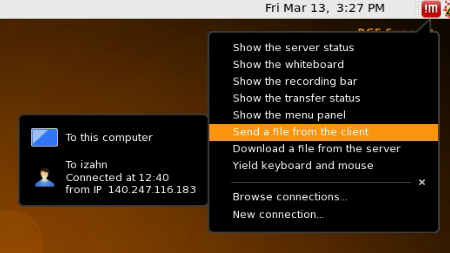
\includegraphics[width=.9\linewidth]{images/NoMachineMenu.png}

If you prefer to transfer files using another file transfer client, anything that uses ssh (e.g., \href{http://filezilla-project.org/}{FileZilla}) should work. Just point your favorite client to \texttt{rce.hmdc.harvard.edu}.

\section{Interactive jobs}
\label{sec-6}
When you first log on to the RCE you are on a \emph{login node}. The login nodes are not designed for intensive computation; the purpose of the login nodes is to provide access to the \emph{interactive nodes} and the \emph{batch nodes}. Interactive jobs are useful when a) you need a lot of memory (e.g., because you need to load a large dataset into memory), and/or b) you want to use multiple cores to speed up your computation.

\subsection{Launching applications on the interactive nodes}
\label{sec-6-1}
Running applications on the interactive nodes is very easy; just log in \hyperref[sec-2]{using NoMachine} and launch your application from the \texttt{Application -{}-> RCE Powered} menu. A dialog will open asking you how much memory you need and how many CPUs, and then your application will open. That's all there is to it! Well, we should say that the RCE is a shared resource, so please try not to request more memory or CPUs than you need. Also, applications running on the interactive nodes will expire after five days; you can request an extension, but if you fail to do so your job will be terminated 120 hours after it starts. For details refer to \url{http://projects.iq.harvard.edu/rce/book/extending-rce-powered-application}.

\subsection{Available RCE powered applications}
\label{sec-6-2}

Available RCE powered applications include:
\begin{itemize}
\item Gauss
\item Mathematica
\item Matlab/Octave
\item R/RStudio
\item SAS
\item Stata (MP and SE)
\item StatTransfer
\end{itemize}

Other applications (e.g., Python/IPython, perl, tesseract, various Unix programs and utilities) can be run on the interactive nodes by launching a terminal on an interactive node (\texttt{Applications -{}-> RCE Powered -{}-> RCE Shell}) and launching your program from the command line.

If you are using the interactive nodes primarily for the large memory they provide you should have all the information you need to begin taking advantage of the RCE. If you are also interested in using multiple CPU cores to speed up your computations, read on! The following sections contain examples illustrating techniques for utilizing multiple cores on the RCE.

\subsection{Using multiple CPUs in R}
\label{sec-6-3}
This section illustrates how to take advantage of multiple cores when running interactive jobs on the RCE. Since memory requirements are easy to satisfy (just specify how much you need when you launch and application via the \texttt{Application -{}-> RCE Powered} menu), the examples presented here will focus on utilizing multiple CPUs. 

There are many different packages for utilizing multiple cores in R, but one of the simplest is the \href{https://stat.ethz.ch/R-manual/R-devel/library/parallel/doc/parallel.pdf}{parallel} package\footnote{For additional packages useful for parallel computing see the \href{http://cran.r-project.org/web/views/HighPerformanceComputing.html}{HPC task view}.}. To use it load the parallel package and use the \texttt{parLapply} function or the \texttt{mclapply} function. 

\subsubsection{Using multiple cores to speed up simulations}
\label{sec-6-3-1}
Running computations in parallel on multiple cores is often an effective way to speed up computations. This can be especially useful when doing simulations, or when using resampling methods such as bootstrap or permutation tests. In this example parallel processing is used to simulate the sampling distribution of the mean for samples of various sizes.

We start by setting up a helper function to repeatedly generate a sample of a given size and calculate the sample mean.
\begin{verbatim}
## function to generate distribution of means for a range of sample sizes
meanDist <- function(n, nsamp = 5000) {
  replicate(nsamp, mean(rnorm(n)))
}

## range of sample sizes to iterate over
sampSizes <- seq(10, 500, by = 5)
\end{verbatim}

Next iterate over a range of sample sizes, generating a distribution of means for each one. This can be slow because R normally uses only one core:
\begin{verbatim}
system.time(means <- lapply(sampSizes, meanDist))
\end{verbatim}

\begin{verbatim}
  user  system elapsed 
33.270   0.020  33.295
\end{verbatim}

The simulation can be carried out much more rapidly using \texttt{mclapply} instead:
\begin{verbatim}
library(parallel) 
system.time(means <- mclapply(sampSizes, meanDist, mc.cores = 7))
\end{verbatim}

\begin{verbatim}
 user  system elapsed 
36.48    1.01    5.68
\end{verbatim}

Like \texttt{lapply} the \texttt{mclapply} function returns a list, which we can process as usual. For example, we can construct histograms of the sampling distributions of the mean that we simulated above:
\begin{verbatim}
## plot the distribution of means at various sample sizes
par(mfrow=c(6, 5), mar = c(0,0,2,2), cex = .7)
for(i in 1:30) {
  hist(means[[i]], 
       main = paste("n =", 
                    sampSizes[i]), 
       axes = FALSE,
       xlim = range(unlist(means)))
}
\end{verbatim}

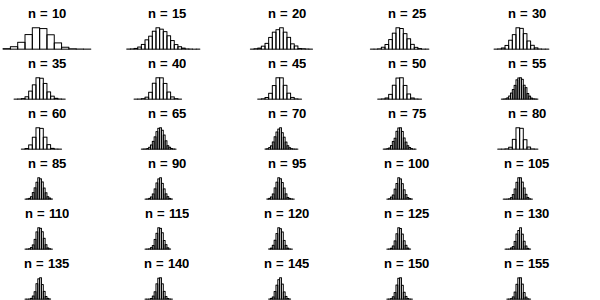
\includegraphics[width=.9\linewidth]{images/samplingDist.png}


\subsubsection{Using multiple cores to speed up computations}
\label{sec-6-3-2}
In the previous example we generated the data on each iteration. This kind of simulation can be useful, but often you want to parallelize a function that processes data from a (potentially large) number of files. This is also easy to do using the parallel package in R. In the following example we count number of characters in all the text files in the texlive directory.
\begin{verbatim}
## List the files to iterate over
textFiles<- list.files("/usr/share/texlive/", 
                       recursive = TRUE, 
                       pattern = "\\.txt$|\\.tex$",
                       full.names = TRUE)

## function for counting characters (NOTE: this example isn't realistic -- it 
## would be better to use the unix "wc" utility if you were doing this
## in real life...)
countChars <-  function(x) {
  sum(nchar(readLines(x, warn = FALSE), type = "width"))
}
\end{verbatim}

We have
\begin{verbatim}
length(textFiles)
\end{verbatim}

\begin{verbatim}
[1] 2087
\end{verbatim}
text files to process. We can do this using a single core:
\begin{verbatim}
system.time(nchars <- unlist(lapply(textFiles, countChars)))
\end{verbatim}

\begin{verbatim}
 user  system elapsed 
27.98    0.29   31.83
\end{verbatim}
but this is too slow. We can do the computation more quickly using multiple cores:
\begin{verbatim}
system.time(nchars <- unlist(mclapply(textFiles, countChars, mc.cores = 7)))
\end{verbatim}

\begin{verbatim}
 user  system elapsed 
26.85    0.68    4.96
\end{verbatim}
and calculate the total number of characters in the text files by summing over the result
\begin{verbatim}
sum(nchars, na.rm = TRUE)
\end{verbatim}

\begin{verbatim}
[1] 31831896
\end{verbatim}

For more details and examples using the parallel package, refer to the \href{https://stat.ethz.ch/R-manual/R-devel/library/parallel/doc/parallel.pdf}{parallel package documentation} or run \texttt{help(package = "parallel")} at the R prompt. For other ways of running computations in parallel refer to the \href{http://cran.r-project.org/web/views/HighPerformanceComputing.html}{HPC task view}.

\subsection{{\bfseries\sffamily TODO} Parallel examples for python, matlab?}
\label{sec-6-4}
I don't know this well enough to write good examples. I tried with python, but couldn't come up with an example where multiple processes was actually faster. Contributions appreciated. --Ista

\subsection{Using multiple CPUs in other programming languages and applications}
\label{sec-6-5}
Using multiple CPU cores in Stata, Matlab and SAS does not require explicit activation -- many functions will automatically use multiple cores if available. For Matlab user-written code can also take advantage of multiple CPUs using the \texttt{parfor} command. Python uses can run multiple processes using the \href{https://docs.python.org/2/library/multiprocessing.html}{multiprocessing} library.

\section{Batch jobs}
\label{sec-7}
The RCE also provides access to a \emph{batch nodes}, a cluster of many lower powered computers. While each individual batch node is not that powerful (each node has one CPU and 4 Gb of memory), there are hundreds of them, and combined they make for a very powerful system indeed. The batch nodes are good for jobs will run for a long time, and for groups of very similar jobs (e.g., simulations where a small number of parameters are varied).

Running jobs on the batch nodes is somewhat more complicated than running interactive jobs on the RCE. The main access points are two \emph{command line} programs, \texttt{condor\_submit\_util} and \texttt{condor\_submit}. \texttt{condor\_submit\_util} prompts you for inputs and uses them to write and submit a \texttt{submit file}. Alternatively, you can write the submit file yourself and submit it using \texttt{condor\_submit}, as shown in the examples below. In this tutorial we focus on writing simple submit files and submitting them with \texttt{condor\_submit}. For more details on automatically generating and submitting using \texttt{condor\_submit\_util} refer to the main \href{http://projects.iq.harvard.edu/rce/book/batch-processing-basics}{RCE batch job documentation}. 

\subsection{Preparing for batch submission}
\label{sec-7-1}

In practical terms, running in "batch" means that you will not be able to interact with the running process. This means that all the information your program needs to successfully complete needs to be specified ahead of time. You can pass arguments to your process so that each job gets different inputs, but the script must process these arguments and do the right thing without further instruction.

When you submit a job to the batch processing system each process will generate output and (perhaps) errors. It is usually a good idea to make a sub-folder to store these results. Thus your project folder should contain at least the following:
\begin{itemize}
\item script or program to run
\item submit file
\item output directory
\end{itemize}

When preparing your job for batch submission you usually need to figure out how to split up the computation, (with one piece going to each process), and how to tell each process which piece it is responsible for. The examples below illustrate how to do this.

\subsection{Submit file overview}
\label{sec-7-2}
In order to run jobs in parallel on the batch nodes you need to create a \texttt{submit file} that describes the process to be run on each node. If creating these files by hand you may use any text editor (e.g., \texttt{gedit}, accessible though the \texttt{Applications -{}-> Accessories} menu on the RCE). 

The submit file template below includes all required elements. (Note that this file is a template only -- see the next section for working examples.)
\begin{verbatim}
# Universe whould always be 'vanilla'. This line MUST be 
#included in your submit file, exactly as shown below.
Universe = vanilla

# Enter the path to the program you wish to run.
# The default runs the R program. To run another
# program just change '/user/local/bin/R' to the
# path to the program you want to run. For example,
# to run Stata set Executable to '/usr/local/bin/stata'.
Executable = /usr/local/bin/R

# Specify any arguments you want to pass to the executable.
Arguments = --no-save --no-restore --slave

# Specify the relative path to the input file (if any). If you
# are using R this should be your R script. If you are using
# Stata this should be your do file.
input = example.R

# Specify where to output any results printed by your program.
output = output/out.$(Process)
# Specify where to save any errors returned by your program.
error = output/error.$(Process)
# Specify where to save the log file.
Log = output/log
# Enter the number of processes to request. This should 
# always be the last part of your submit file.
Queue 10
\end{verbatim}
This submit file instructs the scheduler to request 10 nodes (\texttt{Queue 10}), start R on each one (\texttt{Executable = /usr/local/bin/R}), run the code in example.R (\texttt{input = example.R}), write the output to files named out.0 -- out.9 in the output folder (\texttt{output = output/out.\$(Process)}), write any errors to files named out.0 -- out.9 in the output folder (\texttt{error = output/error.\$(Process)}), and write a log file in the output folder (\texttt{Log = output/log}). 

\subsection{Batch example: Simple power simulation in R}
\label{sec-7-3}
The simplest kind of batch job is one for which you just want to run the same code multiple times, without varying any parameters. For example, suppose that we wish to run a power simulation for a t.test with unequal group sizes. 

\subsubsection{R power simulation script}
\label{sec-7-3-1}
The first step is to write a script or program to carry out the desired computation. The R script below simulates distributions with a specified mean difference, performs two-sample t-tests on the difference, and calculates the proportion of significant tests.
\begin{verbatim}
## function to simulate data and perform a t.test
sim.ttest <- function(mu1, mu2, sd, n1, n2) {
    d <- data.frame(x = c(rep("group1", n1), rep("group2", n2)),
                    y = c(rnorm(n1, mean = mu1, sd = sd),
                          rnorm(n2, mean = mu2, sd = sd)))
    return(t.test(y ~ x, data = d)$p.value)
}

##  run the function 10,000 times 
p <- replicate(10000,
               sim.ttest(mu1 = 1,
                         mu2 = 1.3,
                         sd = 1,
                         n1 = 50,
                         n2 = 150))
## calculate the proportion of significant tests
cat(length(p[p < .05])/length(p))
\end{verbatim}

\begin{verbatim}
[1] 0.4392
\end{verbatim}

\subsubsection{Submit file}
\label{sec-7-3-2}
If we want to run this function one million times it may take a while, especially if our computer is an older less powerful model. So let's run it on 100 separate machines (each one will simulate the test 10000 times). To do that we need, in addition to the R script above, a submit file to request resources and run the computation. 
\begin{verbatim}
# Universe whould always be 'vanilla'. This line MUST be 
#included in your submit file, exactly as shown below.
Universe = vanilla

# Enter the path to the R program.
Executable = /usr/local/bin/R

# Specify any arguments you want to pass to the executable
# to make r not save or restore workspaces, and to 
# run as quietly as possible
Arguments = --no-save --no-restore --slave

# Specify the relative path to the input file
input = power.R

# Specify where to output any results printed by your program.
output = output/out.$(Process)
# Specify where to save any errors returned by your program.
error = output/error.$(Process)
# Specify where to save the log file.
Log = output/log
# Enter the number of processes to request.
Queue 100
\end{verbatim}

Now that we have our script and the submit file we can run submit the job as follows:
\begin{enumerate}
\item make a project folder for this run if it doesn't exist
\item save the R script (as power.R) and the submit file (as power.submit) in the project folder
\item make a sub folder named \texttt{output}
\item open a terminal and \texttt{cd} to the project folder
\item run \texttt{condor\_submit power.submit} to submit the jobs to the cluster
\end{enumerate}

\subsubsection{Monitoring submitted jobs}
\label{sec-7-3-3}
After submitting the jobs we may wish to monitor them, e.g. to check if they are running. You can do this by running \texttt{condor\_q <your\_user\_name>} in a terminal. If this returns nothing then you have no jobs in the queue. Otherwise you will see information for each request in the queue which will look something like this:
\begin{verbatim}
-- Schedd: HMDC.batch@rce6-5.hmdc.harvard.edu : <10.0.0.10:9619?sock=7858_e19e_247>
 ID      OWNER            SUBMITTED     RUN_TIME ST PRI SIZE CMD               
 200.0   izahn           4/27 11:45   0+00:00:04 R  0   0.0  R --no-save --no-r
 200.1   izahn           4/27 11:45   0+00:00:04 R  0   0.0  R --no-save --no-r
 200.2   izahn           4/27 11:45   0+00:00:04 R  0   0.0  R --no-save --no-r
 200.3   izahn           4/27 11:45   0+00:00:04 R  0   0.0  R --no-save --no-r
 200.4   izahn           4/27 11:45   0+00:00:04 R  0   0.0  R --no-save --no-r
 200.5   izahn           4/27 11:45   0+00:00:04 R  0   0.0  R --no-save --no-r
 200.6   izahn           4/27 11:45   0+00:00:04 R  0   0.0  R --no-save --no-r
 200.7   izahn           4/27 11:45   0+00:00:04 R  0   0.0  R --no-save --no-r
 200.8   izahn           4/27 11:45   0+00:00:04 R  0   0.0  R --no-save --no-r
 200.9   izahn           4/27 11:45   0+00:00:04 R  0   0.0  R --no-save --no-r
 200.10  izahn           4/27 11:45   0+00:00:04 R  0   0.0  R --no-save --no-r
 200.11  izahn           4/27 11:45   0+00:00:04 R  0   0.0  R --no-save --no-r
 200.12  izahn           4/27 11:45   0+00:00:04 R  0   0.0  R --no-save --no-r
\end{verbatim}
Perhaps the most important information returned by \texttt{condor\_q} is the program status (the \textbf{ST} column). Status \textbf{I} means your job is in the queue but has not yet started running, \textbf{R} means the job is currently running, and \textbf{H} means the job is on hold. If you job is on hold you can get more information about what the problem might be by running \texttt{condor\_q -hold}.

You will know your job is finished when it is now longer listed in the \texttt{condor\_q} output. When it finishes you can examine the output and/or error files to see if the program exited successfully.

\subsubsection{Aggregating results}
\label{sec-7-3-4}
When your batch job is finished you are usually left with multiple output files that need to be aggregated. In the case of our simulation example, we have files \texttt{output/out.0 -{}- output/out40}, each of which contains a single number representing the proportion of significant tests. We can aggregate them with a simple R script, like this:
\begin{verbatim}
## list all output files in the output directory
output_files <- list.files("output",
                           pattern = "^out\\.[0-9]+$",
                           full.names=TRUE)

## read each file, convert it to a number, and take the average
mean(as.double(sapply(
                      output_files,
                      readLines,
                      warn = FALSE)))
\end{verbatim}

\subsubsection{Try it yourself!}
\label{sec-7-3-5}
Download the \href{examples/power1.zip}{power simulation example files}, to the RCE, extract the zip file and running \texttt{condor\_submit power.submit} in the \texttt{power1} directory.

\subsection{Batch example: Power simulation in R with varying parameters}
\label{sec-7-4}
The previous example was relatively simple, because we wanted to run exactly the same code on all 100 nodes. Often however you want each node to do something slightly different. For example, we may wish to vary the sample size from 100 -- 500 in increments of 10, to see how power changes as a function of that parameter. In that case we need to pass some additional information to each process, telling it which parameter space it is responsible for. 

As it turns out, we almost already know how to do that: if you you look closely at the submit file in the previous example you will notice that we used \texttt{\$(Process)} to append the process number to the output and error files. 
\subsubsection{Submit file passing process as an argument}
\label{sec-7-4-1}
We can use the \texttt{\$(Process)} macro to pass information to our program, like this:
\begin{verbatim}
# Universe whould always be 'vanilla'. This line MUST be 
#included in your submit file, exactly as shown below.
Universe = vanilla

# Enter the path to the R program.
Executable = /usr/local/bin/R

# Specify any arguments you want to pass to the executable
# to make r not save or restore workspaces, and to 
# run as quietly as possible
Arguments = --no-save --no-restore --slave --args $(Process)

# Specify the relative path to the input file
input = power.R

# Specify where to save any errors returned by your program.
error = output/error.$(Process)

Log = log.txt
# Enter the number of processes to request.
Queue 41
\end{verbatim}
Notice that we used \texttt{-{}-args \$(Process)} to pass the process number to the R program. \texttt{\$(Process)} will be an integer starting from \texttt{0}. 

\subsubsection{R script argument processing}
\label{sec-7-4-2}
Next we need to 1) retrieve the process number in our R program and 2) map it to the parameter space. We can retrieve the arguments in R like this:
\begin{verbatim}
## retrieve arguments passed from the command line.
process <- as.integer(as.character(commandArgs(trailingOnly = TRUE)))
\end{verbatim}
We now have a variable in R that tells us which process we are. Now we need to map that to our parameter space; recall that we want to test sample sizes from 100 to 500, so we need to map \texttt{process 0} to \texttt{n = 100},  \texttt{process 1} to \texttt{n = 110}, \texttt{process 2} to \texttt{n = 120} and so on:
\begin{verbatim}
## map process to sample size parameter.
n <- (process + 100) + (process*10 - process)
\end{verbatim}

There is one additional complication we need to handle: in the previous example we did need to keep track of the parameters used by each process because the parameters did not vary. Now that they do, it would be nice if we had output that recorded the value of the varying parameter as well as the result. We could of course just print the \texttt{n} parameter we calculated from the process number along with the result, but it will be easier to combine the outputs if we write them to a machine-readable format (e.g., a comma-separated-values file). You may have noticed that in the submit file above I omitted the \texttt{output} directive: that is because we are going to explicitly save the results in the R script, so we don't need the batch scheduler to save those output files for us.

No we can set up the simulation as before, passing the \texttt{n} calculated above into our simulation function, writing the results to files. 
\begin{verbatim}
  ## function to simulate data and perform a t.test
  sim.ttest <- function(mu1, mu2, sd, n1, n2) {
      d <- data.frame(x = c(rep("group1", n1), rep("group2", n2)),
                      y = c(rnorm(n1, mean = mu1, sd = sd),
                            rnorm(n2, mean = mu2, sd = sd)))
      return(t.test(y ~ x, data = d)$p.value)
  }

  ##  run the function 10,000 times 
  p <- replicate(10000,
                 sim.ttest(mu1 = 1,
                           mu2 = 1.3,
                           sd = 1,
                           n1 = n,
                           n2 = n))
write.csv(data.frame(n = n, power = length(p[p < .05])/length(p)),
          row.names = FALSE,
          file = paste0("output/out", process, ".csv"))
\end{verbatim}

Now we have all the required elements to submit out job, and can do so using \texttt{condor\_submit} as before. 

\subsubsection{Aggregating results}
\label{sec-7-4-3}
When your batch job is finished you are usually left with multiple output files that need to be aggregated. In the case of our simulation example, we have files \texttt{output/out.0 -{}- output/out40}, each of which contains a single number representing the proportion of significant tests. We can aggregate them with a simple R script, like this:
\begin{verbatim}
## list all output files in the output directory
output_files <- list.files("output",
                           pattern = "^out[0-9]+\\.csv$",
                           full.names=TRUE)

## read each file and append them
results <- do.call(rbind, lapply(output_files, read.csv))

## plot
plot(results)
abline(h = 0.8)
\end{verbatim}

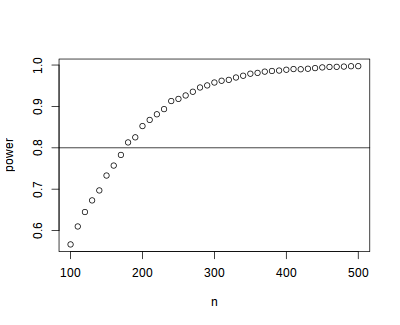
\includegraphics[width=.9\linewidth]{images/powerDist.png}

\subsubsection{Try it yourself!}
\label{sec-7-4-4}
Download the \href{examples/power2.zip}{power simulation example files}, to the RCE, extract the zip file, and run the example by calling \texttt{condor\_submit power.submit} from the \texttt{power2} directory.

\section{{\bfseries\sffamily TODO} Installing custom packages}
\label{sec-8}

\section{{\bfseries\sffamily TODO} Getting help}
\label{sec-9}
% Emacs 24.5.1 (Org mode 8.2.10)
\end{document}